\chapter{Pulse width controlled pulse generator} \label{App:PWCPulseGen}
This appendix presents a VHDL pulse-generator capable of generating different pulse-widths.

The pulse width generator that was described in section \refq{subsec:Pulse_Generator} has been tested.

First, the pulse width of the output was tested. The default pulse width of the module is 40ns and is set in line 3 of code listing \refq{lst:A_PulseGeneratorCode_Entity}. This is the pulse width that will be tested.

\lstinputlisting[language=C ,style = c,firstnumber=1, linerange=34-43, caption={Entity declaration of the pulse generator}, label={lst:A_PulseGeneratorCode_Entity}]{Sections/7_SystemDesign/Code/pulse_width_gen.vhd}

The pulse generators 'o\_pulse' output is connected to an FPGA output pin and the 'i\_master\_clk' signal is a \SIQ{200}{\mega\hertz} CLK signal. The 'i\_trigger' input is connected to a \SIQ{1}{\mega\hertz} internal CLK. The output of the pulse generator can be seen on figure \refq{fig:A_PulseGenWidth_WidthTest}.

\begin{figure}[H]
    \centering
    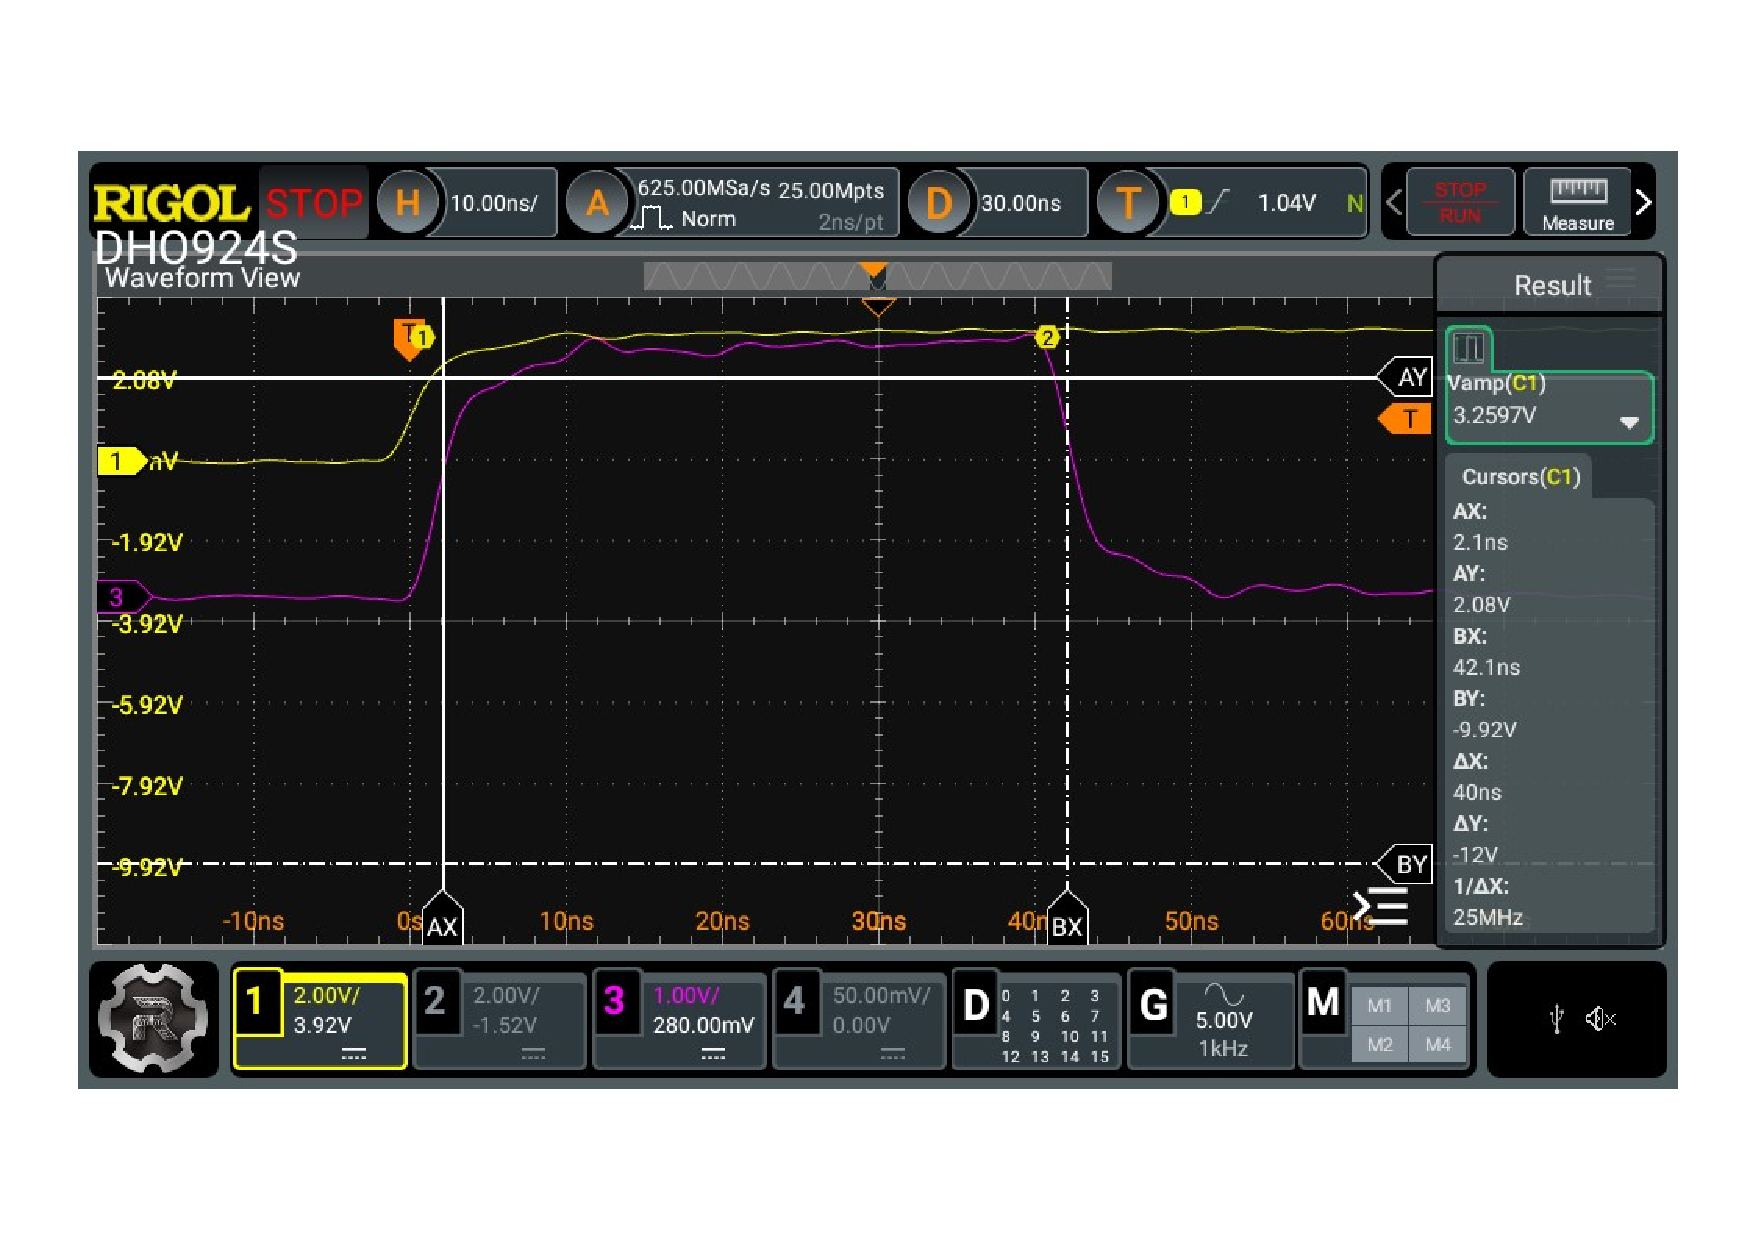
\includegraphics[clip, trim=0 50 0 50, width=1\textwidth]{Appendix/Figures/A_PulseWidthGen_PulseWidth.pdf}
    \caption{An oscilloscope screenshot of the pulse generators output a long with the trigger input. The yellow signal is the trigger input and the purple signal is the pulse generators output. With \SIQ{10}{\nano\second} per division the pulse width is \SIQ{40}{\nano\second} as expected.}
    \label{fig:A_PulseGenWidth_WidthTest}
\end{figure}

The jitter of the pulse generator has also been verified. To do this the trigger input and pulse generator output was measured with an oscilloscope. The oscilloscope is a Rigol DHO924S and it was set to use one of it's 'deep memory' functions, called Ultra Acquire, in order to display several waveforms side by side. The pulse generator is set to produce 40 ns pulses and the results of this can be seen on figure \refq{fig:A_PulseGenWidth_JitterTest}.

\begin{figure}[H]
    \centering
    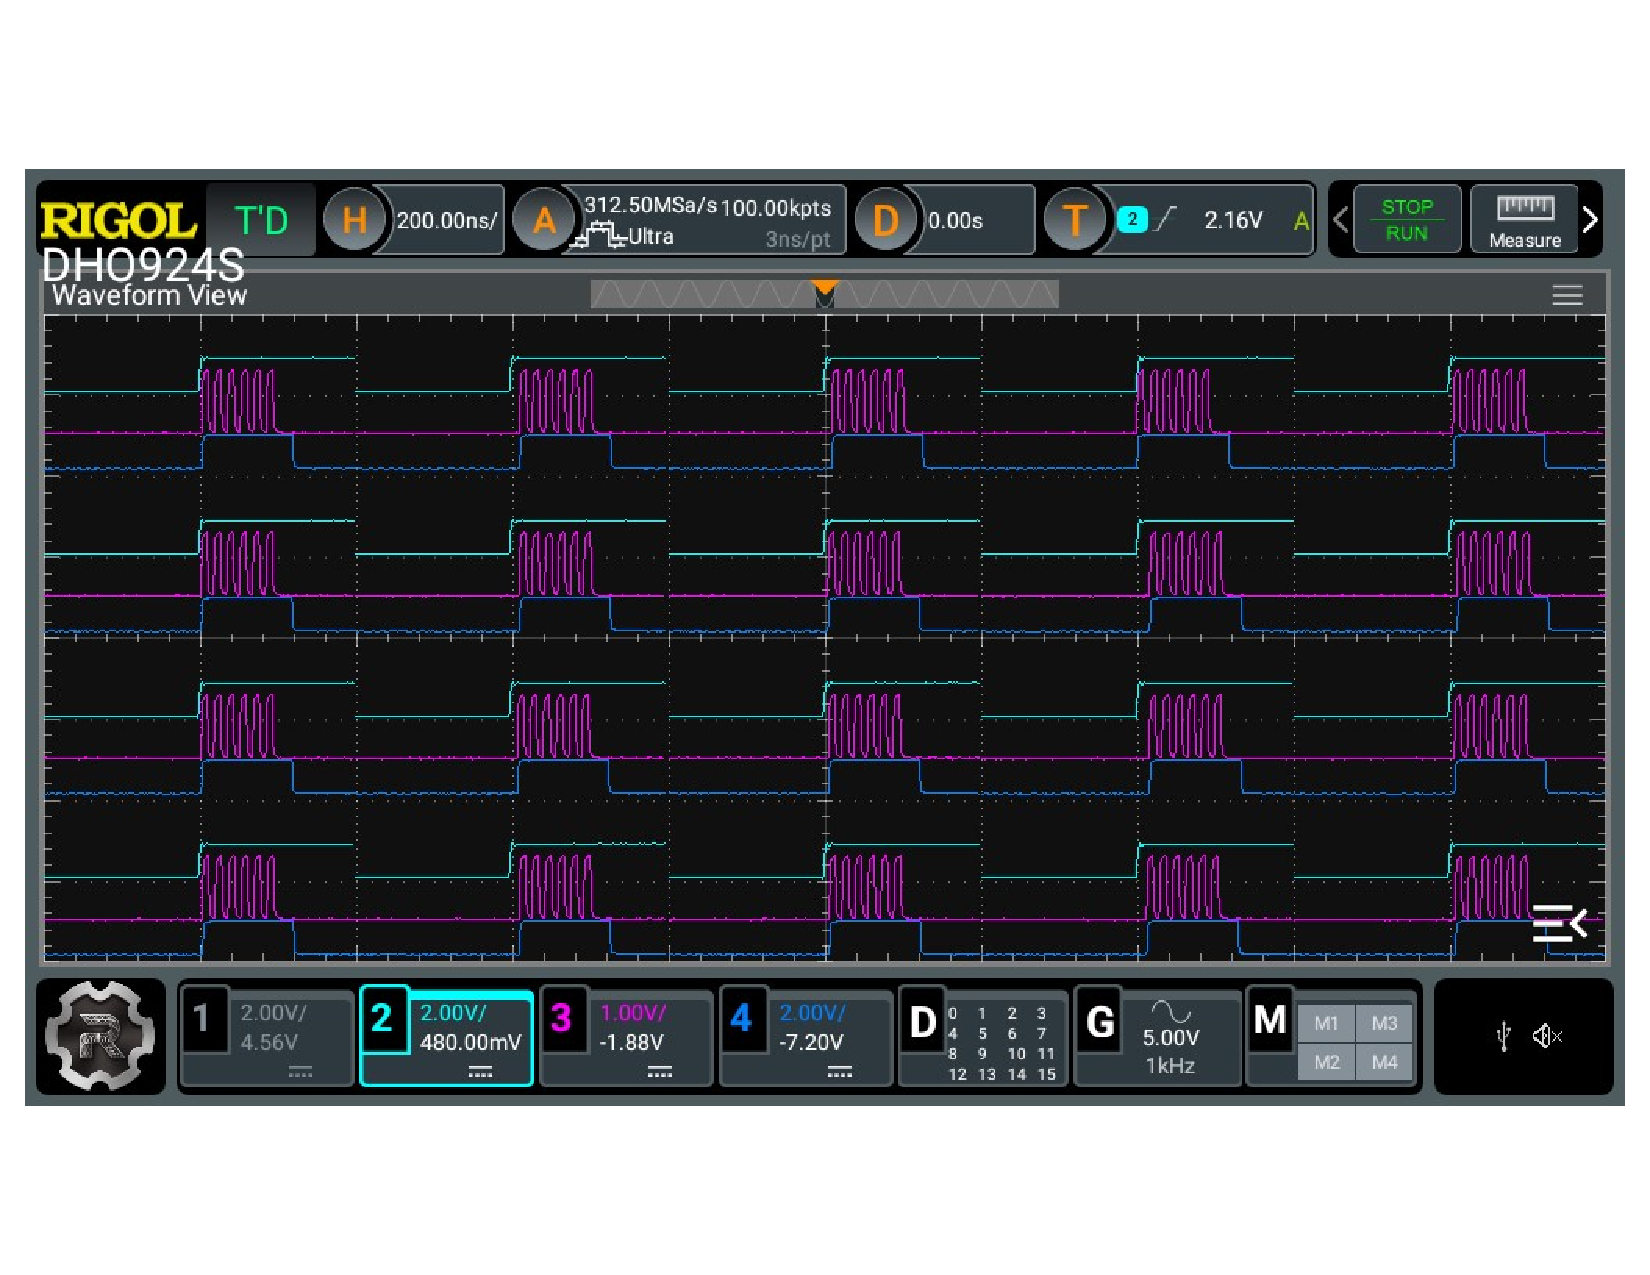
\includegraphics[clip, trim=0 50 0 50, width=1\textwidth]{Appendix/Figures/A_PulseGen_Test.pdf}
    \caption{An oscilloscope screenshot of the pulse generators 'trigger' input (yellow) and 'pulse' output(red). The oscilloscope is using a deep memory 'ultra acquire' mode to display 20 consequtive readings in a 'mosaic' pattern.}
    \label{fig:A_PulseGenWidth_JitterTest}
\end{figure}

It can be seen that, unlike the old pulse generator seen in appendix \refq{App:PulseGenTest}, there appears to be no visible, or varying, delays between the pulse generators activation and the pulse output.

The jitter was measured in another way as well. The pulse generator is set to be retriggered continously, and, since it is expected that the ADC control will take up to 20000 samples at a maximum sample rate of 1MS/s, a delay was added to the oscilloscope in order to see the jitter after 20ms have passed. This delay can be seen on figure \refq{fig:A_PulseGenWidth_JitterTestA}.

\begin{figure}[H]
    \centering
    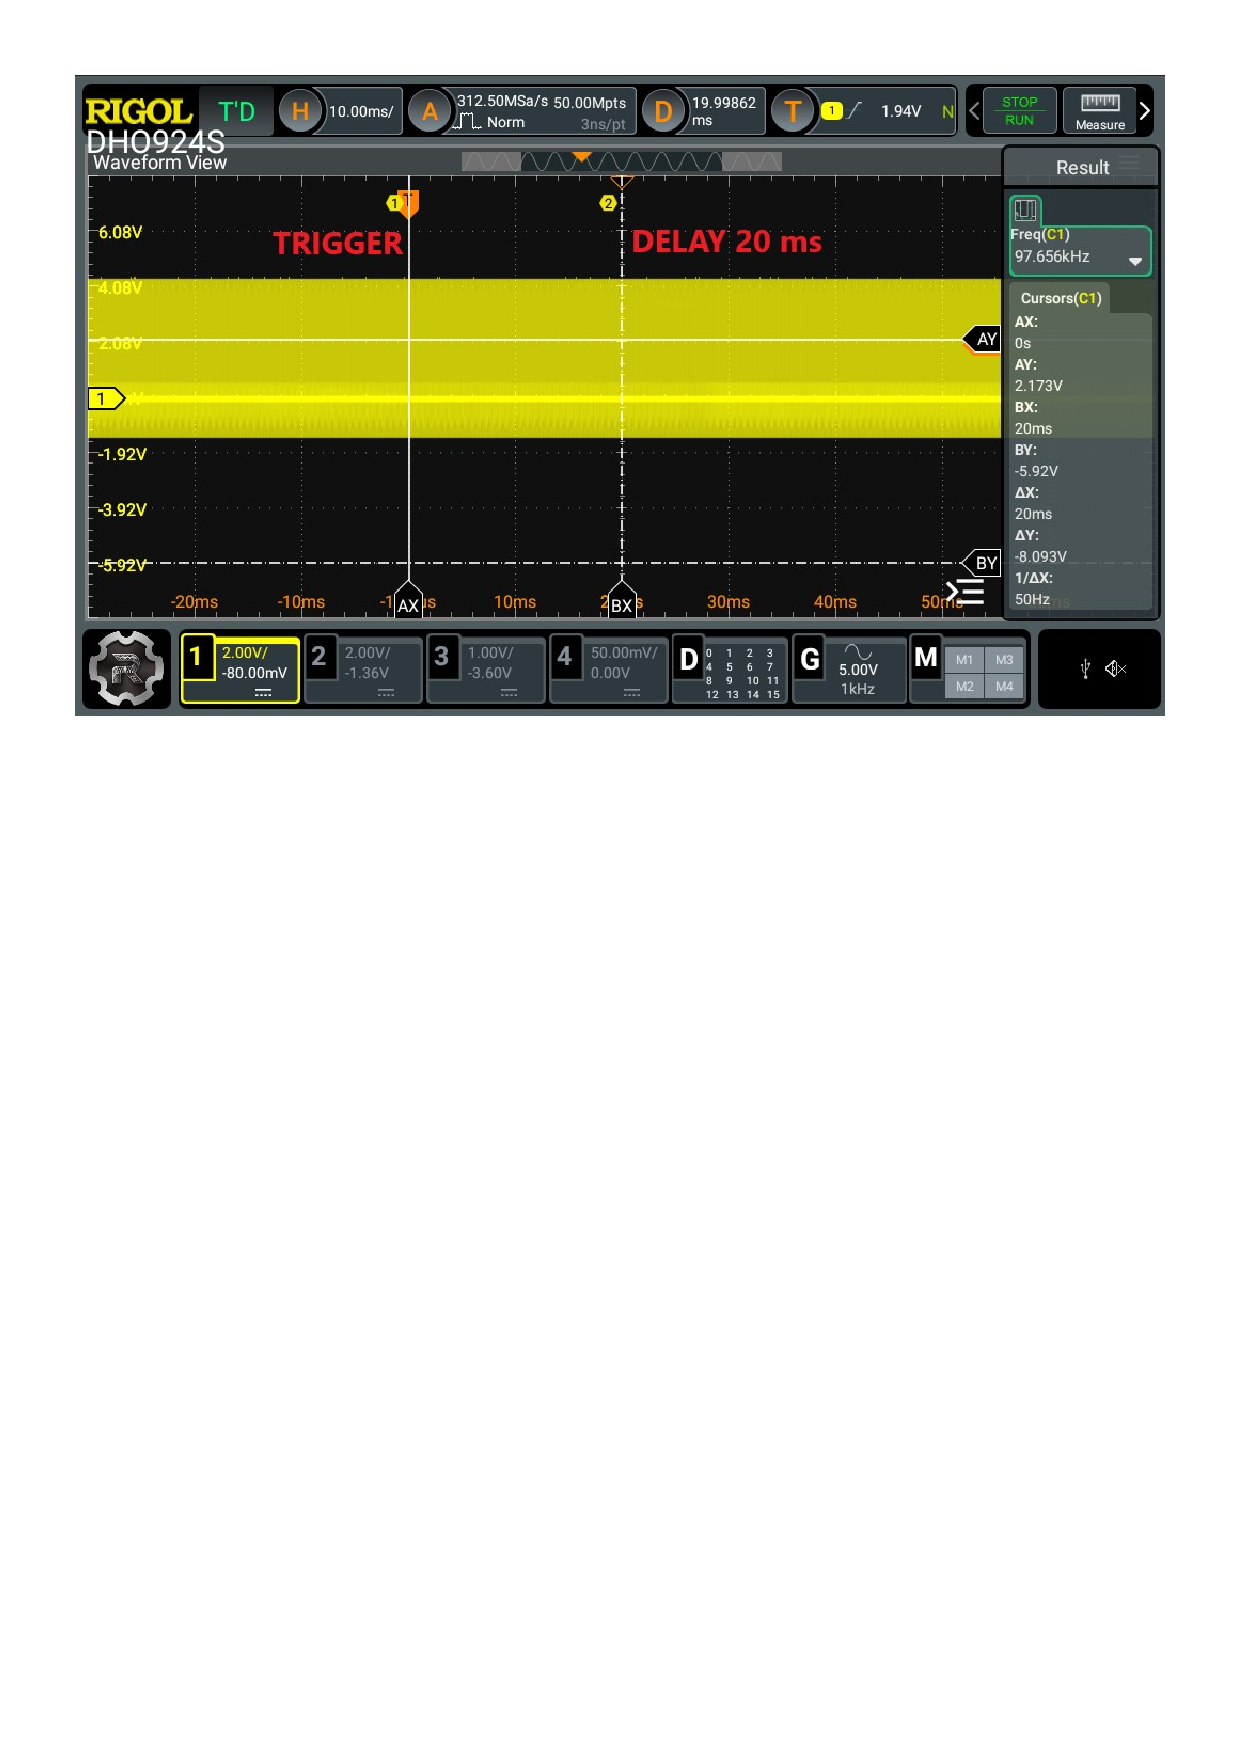
\includegraphics[clip, trim=0 50 0 50, width=1\textwidth]{Appendix/Figures/A_PulseWidthGen_JitterA.pdf}
    \caption{The oscilloscope settings used to measure the jitter. A 20ms delay is added ot the oscilloscope trigger in order to see the 20000th pulse relative to the first pulse.}
    \label{fig:A_PulseGenWidth_JitterTestA}
\end{figure}

Setting the oscilloscope to use maximum persistence it is possible to see the amount of jitter at the 20000th pulse. The result of this can be seen on figure \refq{fig:A_PulseGenWidth_JitterTestB}.

\begin{figure}[H]
    \centering
    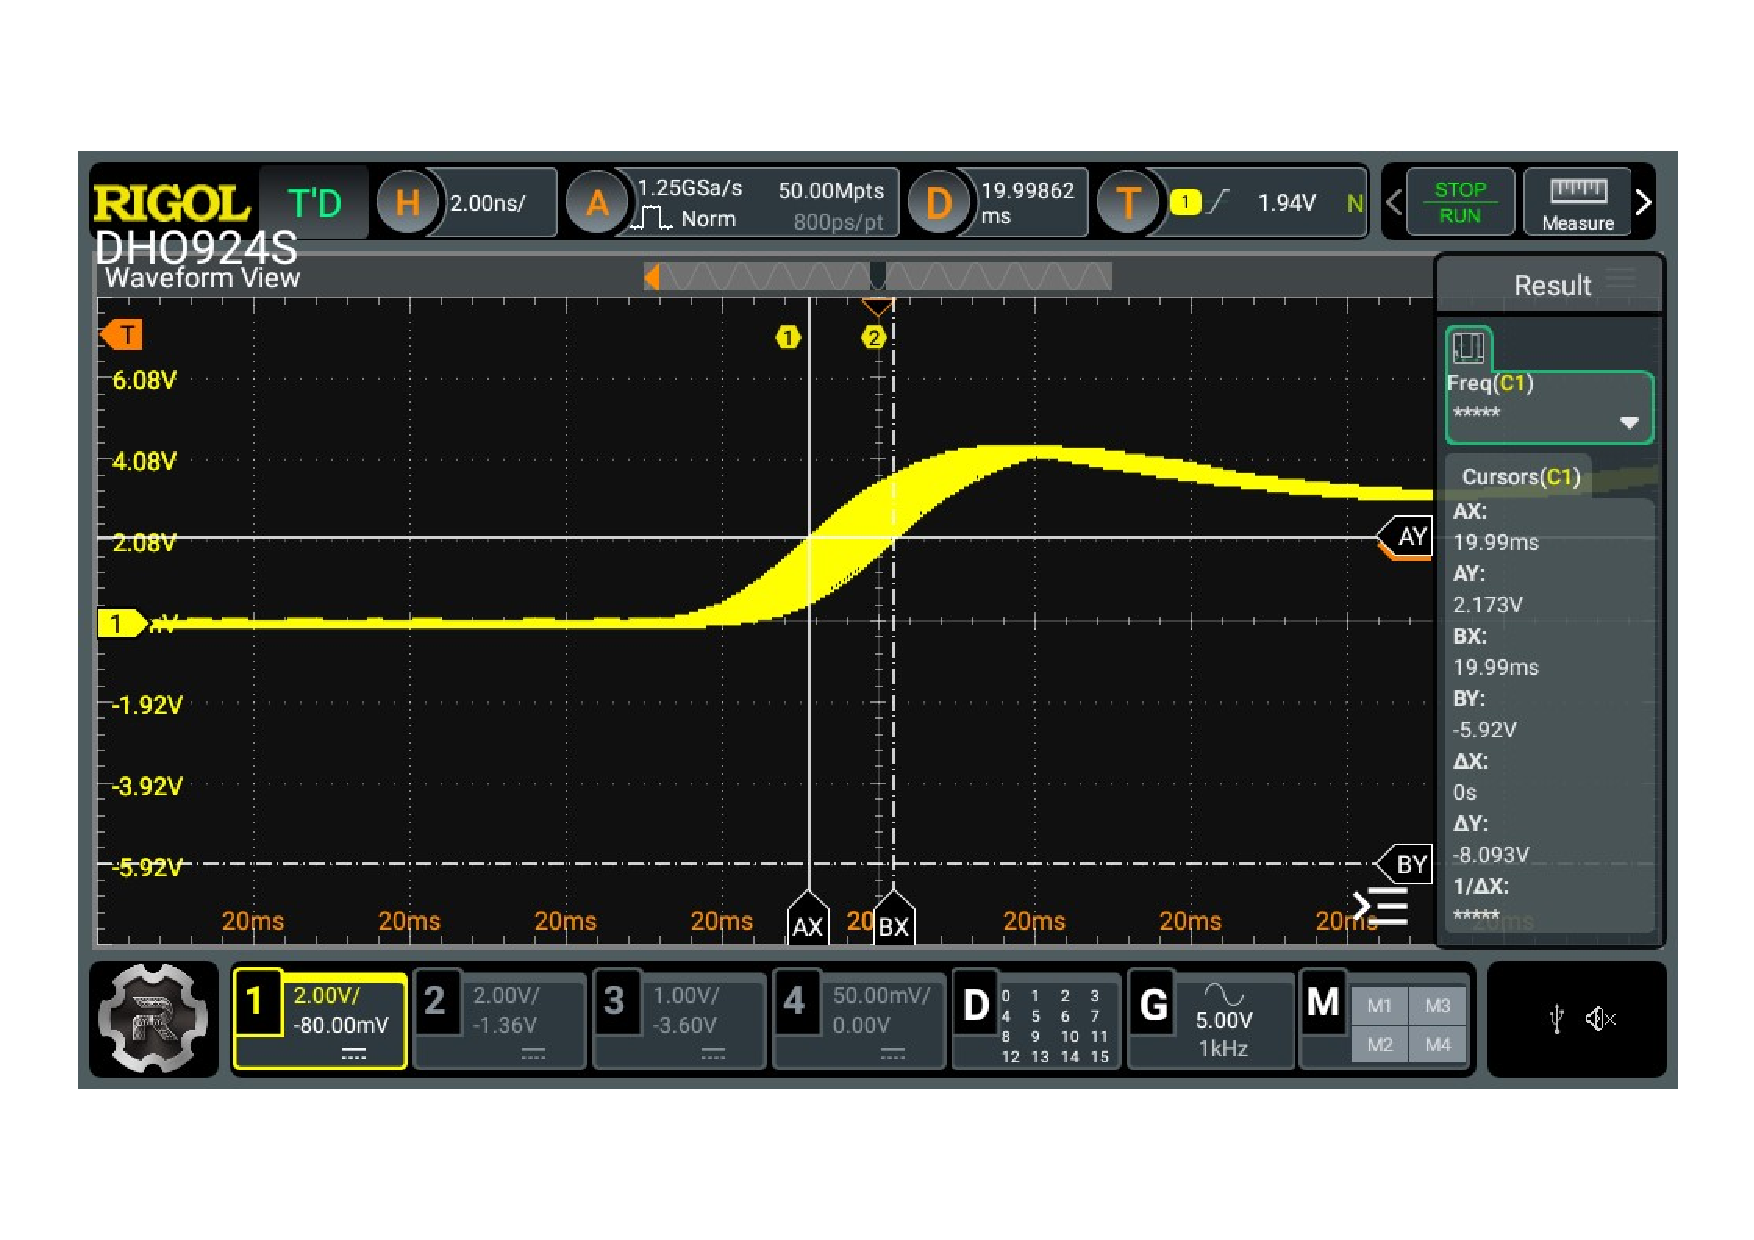
\includegraphics[clip, trim=0 50 0 50, width=1\textwidth]{Appendix/Figures/A_PulseWidth_Gen_JitterB.pdf}
    \caption{A measurement of the jitter of the output of the pulse generator. It is measurably <\SIQ{1}{\nano\second} after 20000 cycles.}
    \label{fig:A_PulseGenWidth_JitterTestB}
\end{figure}

There is little jitter as can be seen on figure \refq{fig:A_PulseGenWidth_JitterTestB}. The oscilloscope is set to \SIQ{2}{\nano\second} per division and the jitter is less than half a division, so, <\SIQ{1}{\nano\second}. This pulse generator can be used for generating CNV pulses.
